\chapter{Frontend Electronic of the Scintillating Fiber Hodoscope}\label{cha:frontend}

%table of slow control register has to be checked
%DAC output voltage (\SI{5}{\volt}) has to be understood
\noindent
\section{Field Programmable Gate Arrays (FPGA)}\label{sec:FPGA}
The frontend electronics for the scintillating fiber hodoscope (SFH) are based on Field Programmable Gate Arrays (FPGAs).
Field Programmable Gate Arrays (FPGAs) are integrated circuits that can be programmed after manufacturing.
FPGA are made up of a grid of programmable logic blocks (PLBs) and programmable interconnects.
They possess the advantage of being flexible, reconfigurable and able to process large amounts of data in parallel.
The frontend electronics for the SFH require large amounts of data to be processed in real time, which makes FPGAs, with their large data throughput and parallel processing capabilities, ideal for this task.\autocite{FPGA_reviewDSP}
\newline
The FPGA used in the frontend electronics for the scintillating fiber hodoscope is part of the Xilinx Artix-7 family.\autocite{InternalcommunicationIgor}
\section{Overview of the Frontend Electronics}
\begin{figure}[h]
    \centering
    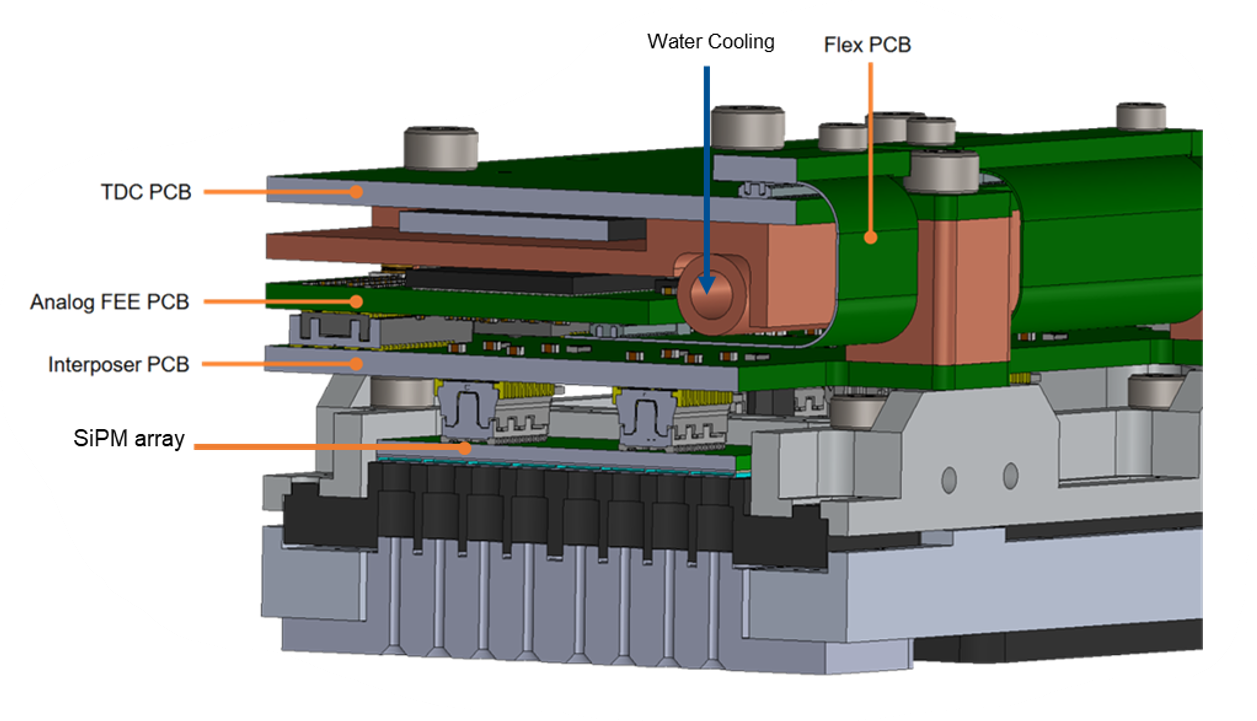
\includegraphics[width=0.9\textwidth]{FrontendAngluarview.png}
    \caption{Sideview of the frontend electronics that will be attached on the sides of the SFH, the fiber holders will be attached to the fibers.\autocite{InternalcommunicationKarl} }
    \label{fig:SideviewModelElectronics}
    \end{figure}
\subsection{Processing of the SFH Signal}
The frontend electronics of the scintillating fiber hodoscope process the signals from the scintillating fibers.
They are attached on all four sides of the SFH, as shown in Figure \ref{SFHpicture}.
\newline 
Two types of readout are considered for the SFH, a mirrored readout and a non-mirrored readout.
In the mirrored scenario, only one end of the fibers is connected to the SiPM array and the other end is mirrored,
while in the non mirrored readout, both ends are connected.\autocite{InternalcommunicationKarl}
\newline
The mirrored scenario has the advantage of only requiring 4 instead of 8 frontend electronics units, halving the number of channels and thus the amount of data that has to be processed.
Furthermore, test beam measurements show that the mirrored readout has a higher efficiency than the non-mirrored readout.\autocite{InternalcommunicationIgor}
\newline
Due to these advantages, currently, the mirrored configuration is planned for the SFH.\autocite{InternalcommunicationKarl}
\newline
Each SFH possesses 768 fibers, for the mirrored configuration, this results in 768 signals that have to be processed, spread out over 4 frontend electronics units, each handling 192 signals. 
\newline
The fibers are connected to the fiber holders as shown in Figure \ref{fig:SideviewModelElectronics}.
The incoming photons are converted into electric signals by the SiPM arrays.
\newline
These are then transmitted to the heart of the frontend electronics via the interposer PCB, also shown in Figure \ref{fig:SideviewModelElectronics}.
\newline
The heart of the frontend electronics is made up of two components, the FEE PCB and iFTDC, stacked on top of each other,
connected by three flex PCBs and plug connectors.
\newline
\begin{figure}[H]
    \centering
    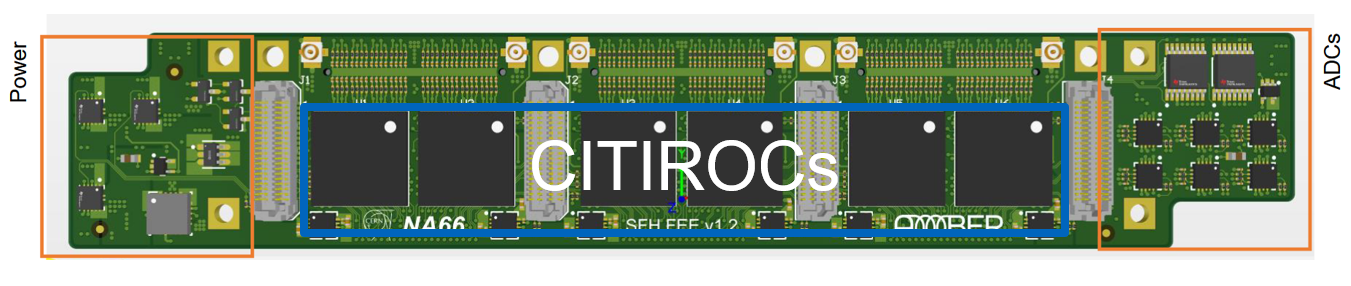
\includegraphics[width=0.6\textwidth]{beschrifteterFEE.png}
    \caption{The analog frontend electronics (FEE) PCB with the six Citiroc1A ASICs.
    The output of the Citiroc1A ASICs is transmitted to the iFTDC over three flex PCBs.\autocite{InternalcommunicationKarl}}
    \label{fig:FEE}
\end{figure}
The analog frontend electronics (FEE) PCB, illustrated in Figure \ref{fig:FEE}, incorporates six Citiroc1A ASICs, each handling 32 channels.
The SiPM signals are amplified, shaped and dicsriminated by the Citiroc1A ASICs  and then transmitted to the iFTDC over the three flex PCBs.
\newline
The FPGA housed on the iFTDC, described in Section \ref{sec:iFTDC},
reads these signals out and processes them, as well as controlling the Citiroc1A ASICs with the signals shown in Figure \ref{fig:FPGA_sigs}.\autocite{InternalcommunicationIgor}
\begin{figure}[H]
    \centering
    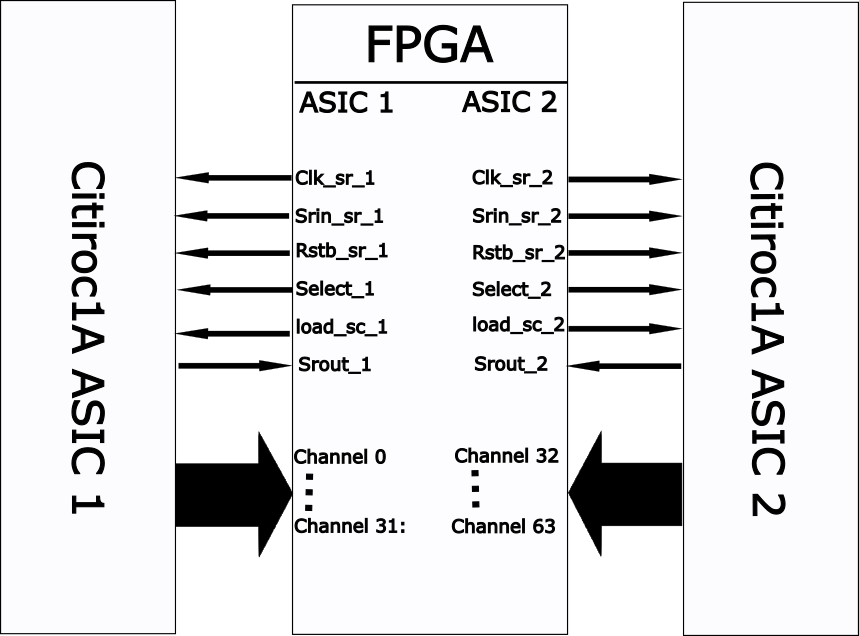
\includegraphics[width=0.7\textwidth]{FPGA_sig.png}
    \caption{The signals used by the FPGA to control and readout the two Citiroc1A ASICs.\autocite{datasheetCITIROC}}
    \label{fig:FPGA_sigs}
\end{figure}


\section{The Citiroc1A ASIC}
The Citiroc1A ASIC is an Application-Specific Integrated Circuit developed by Weeroc company for the readout of SiPM detectors.
It allows for the readout of 32 channels and is sensitive to $\frac{1}{3}$ of a photoelectron.\autocite{datasheetCITIROC}
\subsection{Signal Processing of the Citiroc1A}
\begin{figure}[h]
    \centering
    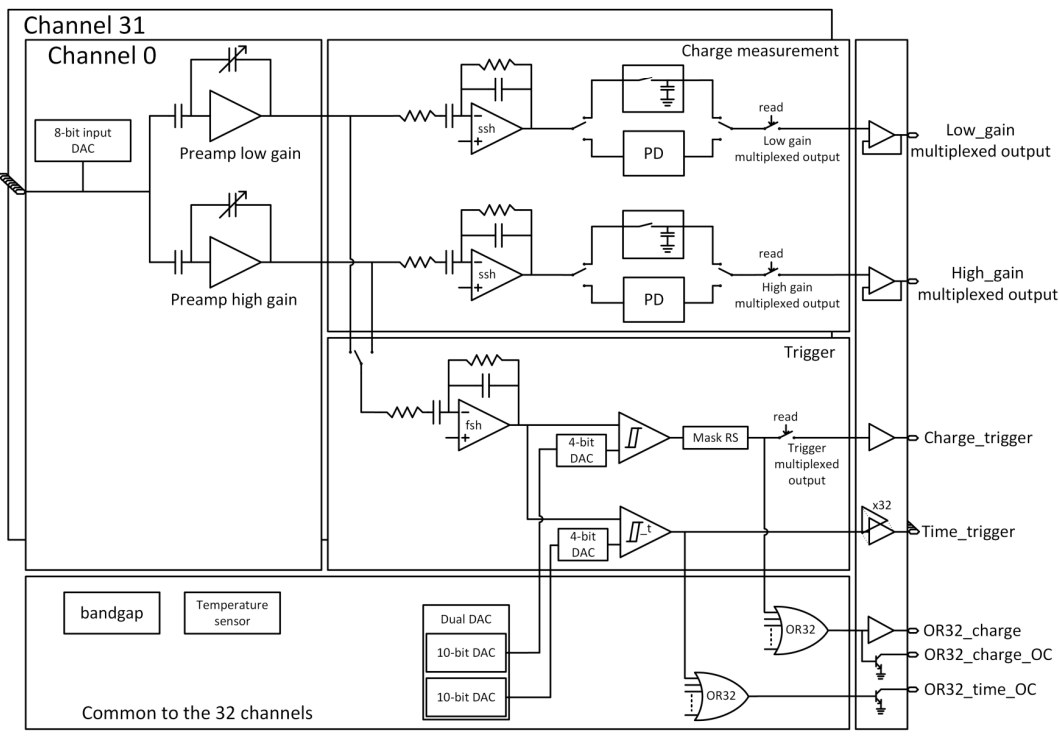
\includegraphics[width=0.8\textwidth]{TRIGER.PNG}
    \caption{General ASIC block scheme of the Citiroc1A.\autocite{datasheetCITIROC}}
    \label{fig:CITIROC1A_TRIGEER}
\end{figure}

The general block scheme of the Citiroc1A is shown in Figure \ref{fig:CITIROC1A_TRIGEER}.
\newline
The Citiroc1A allows fine tuning of the SiPM bias voltage for each channel via the 8-bit input DAC.
\newline	
The input signals are amplified with a for every channel configurable high or low gain by an integrator as depicted in Figure \ref{HighGain}.
\begin{figure}[h]
    \centering
    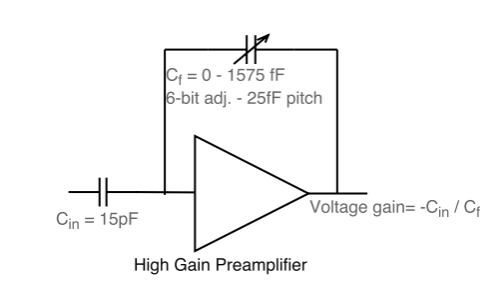
\includegraphics[width=0.8\textwidth]{HighGain.PNG}
    \caption{High gain amplification of the Citiroc1A. The feedback capacitance is adjustable from \SI{25}{\femto\farad} to \SI{1575}{\femto\farad} in \SI{25}{\femto\farad} steps.\autocite{datasheetCITIROC}}
    \label{HighGain}
\end{figure}
The feedback capacitance of for the high gain is adjustable from \SI{25}{\femto\farad} to \SI{1575}{\femto\farad} in \SI{25}{\femto\farad} steps, via a 6 bit dac, with the feedback capacitance following equation \ref{eq:gain}
\begin{equation}
    \text{feedback capacitance} = (63 - \text{Dac\_value}) \times \SI{25}{\femto\farad}
    \label{eq:gain}
\end{equation}
and the resulting voltage amplification equation \ref{eq:voltage_amplification} 
\begin{equation}
    \frac{V_{\text{out}}}{V_{\text{in}}} = \frac{\SI{15}{\pico\farad}}{\text{feedback capacitance}} = 600 \times \frac{1}{63 - \text{Dac\_value}}
       \label{eq:voltage_amplification}
   \end{equation}
\autocite{datasheetCITIROC}

The PRM experiment requires the maximal high gain of 62 amplifying the incoming voltage by a factor 600.\autocite{InternalcommunicationIgor}
\newline
The amplified signals are then shaped by either the slow (ssh) or fast shaper (fsh), as shown in Figure \ref{fig:CITIROC1A_TRIGEER}. 
The fast shaper is used for the PRM experiment since it has a better time resolution, which is important for the SFH performance.\autocite{datasheetCITIROC}
\newline
Each channel of the ASIC has two discriminators, namely the charge discriminator and the time discriminator. In this thesis, i discuss only the time discriminator,
since it provides the time information.
The time discriminator threshold is adjustable via a 10-bit dac for all channels and an additional 4-bit dac for every channel individually, as shown in Figure \ref{fig:CITIROC1A_TRIGEER}\autocite{datasheetCITIROC}.

\subsection{Configuration of the Citiroc1A}\label{sec:configuration}
\begin{figure}[h]
    \centering
    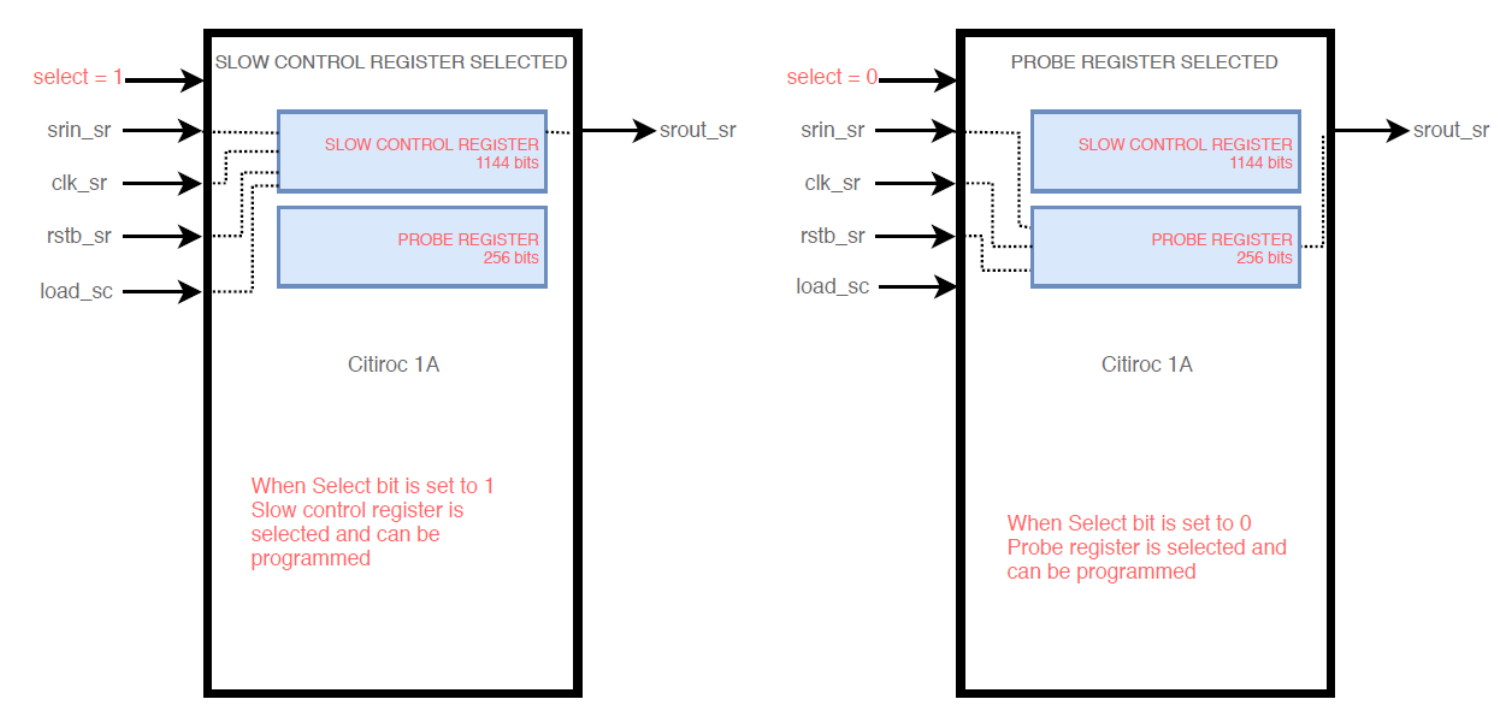
\includegraphics[width=0.8\textwidth]{CitirocConfigHighqual.png}
    \caption{The two configurable registers of the Citiroc1A are selected using the \textcolor{red}{Select} signal. 
    The FPGA communicates with the Citiroc1A through the signals \textcolor{red}{Clk\_sr}, \textcolor{red}{Rstb\_sr}, 
    \textcolor{red}{Srin\_sr}, and \textcolor{red}{Load\_sr}, while the \textcolor{red}{Srout} signal is sent back from the Citiroc1A to the FPGA for verification.\autocite{datasheetCITIROC}}
    \label{fig:CITIROC1A_config}
\end{figure}
The configuration of the Citiroc1A is achievd by the FPGA via the five signals shown in Figure \ref{fig:CITIROC1A_config}.
The \textcolor{red}{Select} signal allows the choice between configuring the slow control, for \textcolor{red}{Select} = 1  or the probe register, for \textcolor{red}{Select} = 0.\autocite{datasheetCITIROC}

\subsubsection{The Slow Control Register}

\begin{figure}
    \centering
    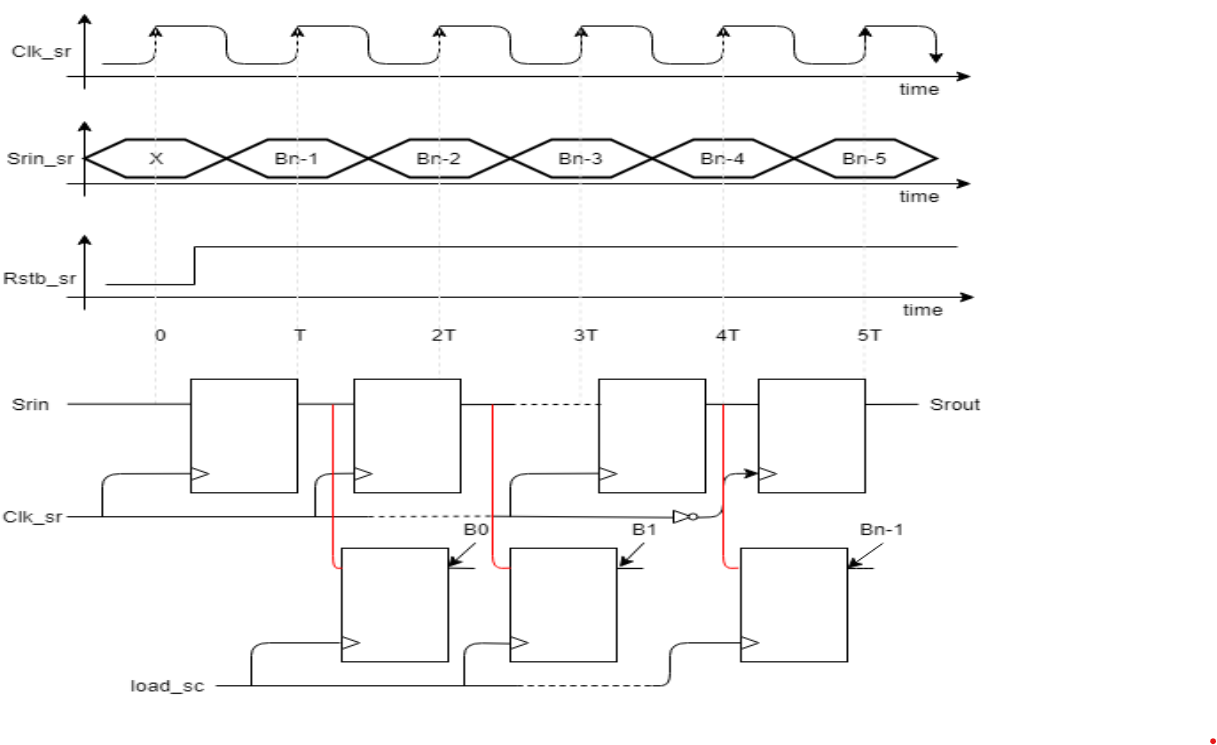
\includegraphics[width=0.8\textwidth]{BitwriteSlowControl.png}
    \caption{The slow control chronogram, depicting the bitstream writing process controlled by  \textcolor{red}{Clk\_sr} the clock signal and  \textcolor{red}{Srin\_sr} the data signal. A rising edge of \textcolor{red}{Load\_sr} is required
     after successful verification with the \textcolor{red}{Srout} signal to load the slow control register.\autocite{datasheetCITIROC}}
    \label{fig:CITIROC1A_writing_bitstream}
\end{figure}
The slow control register is used to set values for internal variables like the high gain for a channel or the time discriminator threshold.
It also allows the FPGA to turn off specific stages of the Citiroc1A, such as the slow shaper or the time discriminator.
The register is 1144 bits long. A complete list of all the registers of the slow control is shown in Table \ref{tab:slow_control_register} in Appendix \ref{cha:Citiroc1A_register}.
\newline
The process of writing the bitstream into the slow control register by the FPGA is illustrated in Figure \ref{fig:CITIROC1A_writing_bitstream}.
\newline
The \textcolor{red}{Rstb\_sr} signal is an asynchronous active-high reset for the serial register, applying to both the slow control and probe register. 
\newline
The FPGA processes the bitstream sequentially, starting with the least significant bit (LSB).
The first bit of the bitstream to enter the serial register will be the last bit of the slow control register.
Each bit is sent on the \textcolor{red}{Srin\_sr} signal in coordination with a rising edge of the \textcolor{red}{Clk\_sr} clock signal.
\newline
The \textcolor{red}{Load\_sr} signal is used to load the bitstream into the slow control register. After all bits have been sent to the Citiroc1A,
a rising edge on \textcolor{red}{Load\_sr} is required to load the slow control register.
\newline
The \textcolor{red}{Srout} signal is sent back from the Citiroc1A to the FPGA for bitstream verification.
Only after the FPGA has sent the full bitstream twice does the \textcolor{red}{Srout} signal take on the value of the bitstream, since the \textcolor{red}{Srout} signal is shifted by the length of the bitstream.\autocite{datasheetCITIROC}
One should only set the rising edge of the \textcolor{red}{Load\_sr} signal after verifying that the \textcolor{red}{Srout} signal takes on the correct values.

\subsubsection{The Probe Register}\label{sec:probe_register}
\begin{figure}[H]
    \centering
    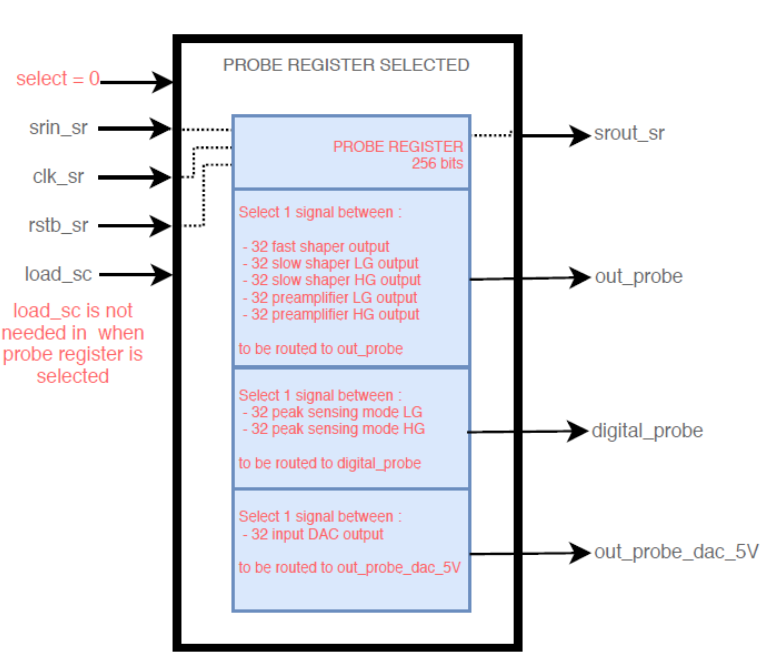
\includegraphics[width=0.8\textwidth]{ProbeRegister.png}
    \caption{Scheme block of internal probing system, allowing the routing of internal signals to probe pins for debugging purposes. It is configured via the probe register.\autocite{datasheetCITIROC}}
    \label{fig:CITIROC1A_proberegiseter}
\end{figure}
The probe register is used to route internal signals to several output pins for debugging purposes.
Its functionality is illustrated in Figure \ref{fig:CITIROC1A_proberegiseter}.
The register consists of 256 bits and is written the same way as the slow control register,
 with the difference that the bits are directly written into the Citiroc1A without requiring a rising edge on \textcolor{red}{Load\_sc}.\autocite{datasheetCITIROC}
\newline
 The complete list of the probe register is shown in Table \ref{tab:probe_register_tab} in Appendix \ref{cha:Citiroc1A_register}.
\newline
The internal signals for each channel that can be routed to the output pins are shown in Table \ref{tab:probe_register}. 
 \begin{table}[H]
    \centering
    \begin{tabular}{@{}lll@{}}
    \toprule
    \textbf{Signal Source} & \textbf{Description}                   & \textbf{Output Pin}        \\ \midrule
    High and low gain preamplifier, & Outputs of preamplifiers and shapers & \texttt{out\_probe}        \\
    slow and fast shapers                                                   &                          \\ \midrule
    \texttt{PeakSensing\_modeb\_LG} & Internal peak-sensing signal for low gain & \texttt{digital\_probe}    \\
    \texttt{PeakSensing\_modeb\_HG} & Internal peak-sensing signal for high gain & -    \\ \midrule
    Output of input DAC            & DAC output voltage (\SI{5}{\volt})  & \texttt{out\_probe\_dac\_5\_V} \\ \bottomrule
    \end{tabular}
    \caption{Internal signal routing to output pins for each channel.}
    \label{tab:probe_register}
\end{table}
Only one signal can be routed to each output pin at a time without potentially causing a short circuit.\autocite{datasheetCITIROC}
\subsection{The iFTDC}\label{sec:iFTDC}
\begin{figure}[H]
    \centering
    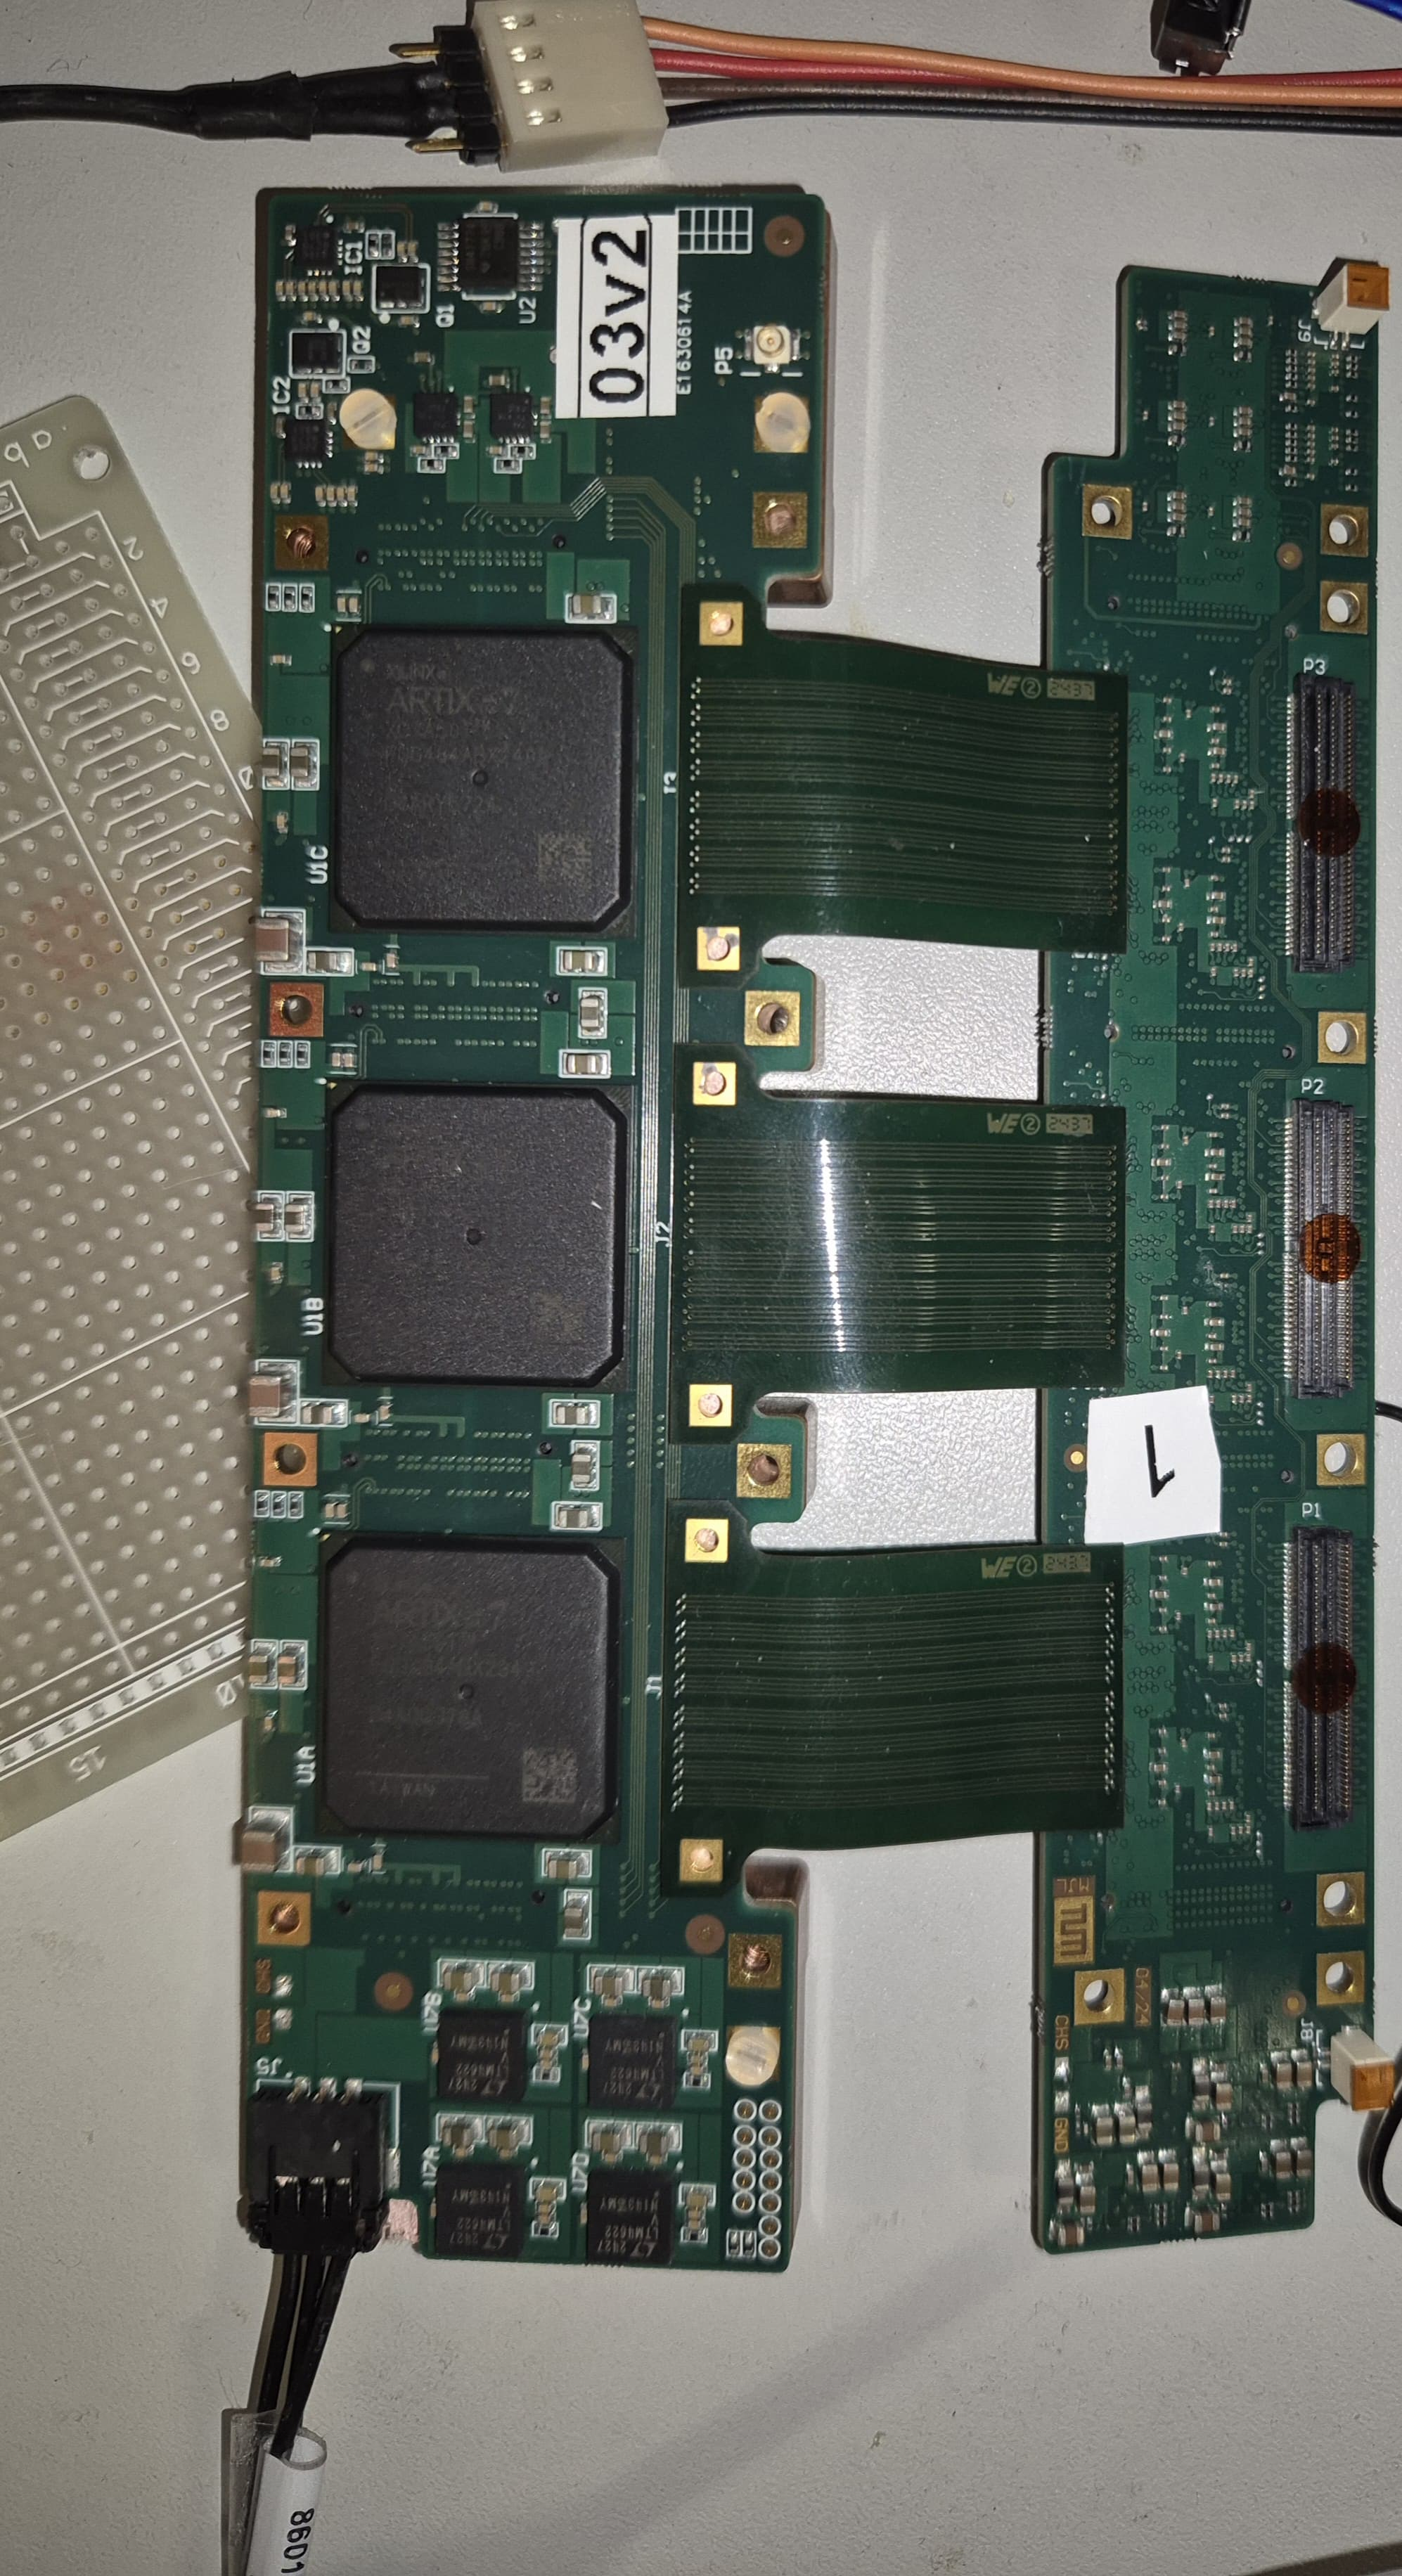
\includegraphics[width=0.5\textwidth]{WhatsApp Bild 2024-12-06 um 12.54.12_a1c66d92.jpg}
    \caption{The iFTDC with three Artix-7 FPGA, the three flex PCBs that connect the iFTDC with the FEE PCB and the connected power supply.}
    \label{fig:iFTDC}
\end{figure}

The iFTDC, depicted in Figure \ref{fig:iFTDC}, is a FPGA based time-to-digital converter. It houses three Artix-7 FPGA.
Each FPGA handles the readout as well as the control  of two of the Citiroc1A ASICs.\autocite{InternalcommunicationIgor}
\newline
The FPGA firmware is loaded via jtag. The control and readout of the FPGAs is performed via Ethernet.









 

